\section{Greedy Deployment}
\label{sec:greedy_deployment}

The \textit{greedy deployment} scheme selects the largest reactor first until another
reactor exceeds the demand---as outlined in \ref{fig:greedy_diagram}. Then, it moves to the next largest reactor until the next deployment of the smallest capacity reactor exceeds the demand. This scheme is not a proxy for strategic decisions by individual actors, but it reveals the implications of deploying a minimal number of reactors to meet the demand.

Previous work from Bachmann et al. \cite{bachmann_enrichment_2021} employed a similar scheme to explore the deployment of advanced reactors in the \gls{usa}. Both implementations are computationally efficient and allow for the exploration of the deployment of advanced reactors in a way that is not overly complex. This scheme is most useful for scenarios where the user is interested in comparing metrics relative to the number of specific reactors deployed outside of the context of the problem.

\begin{figure}[H]
    \centering
    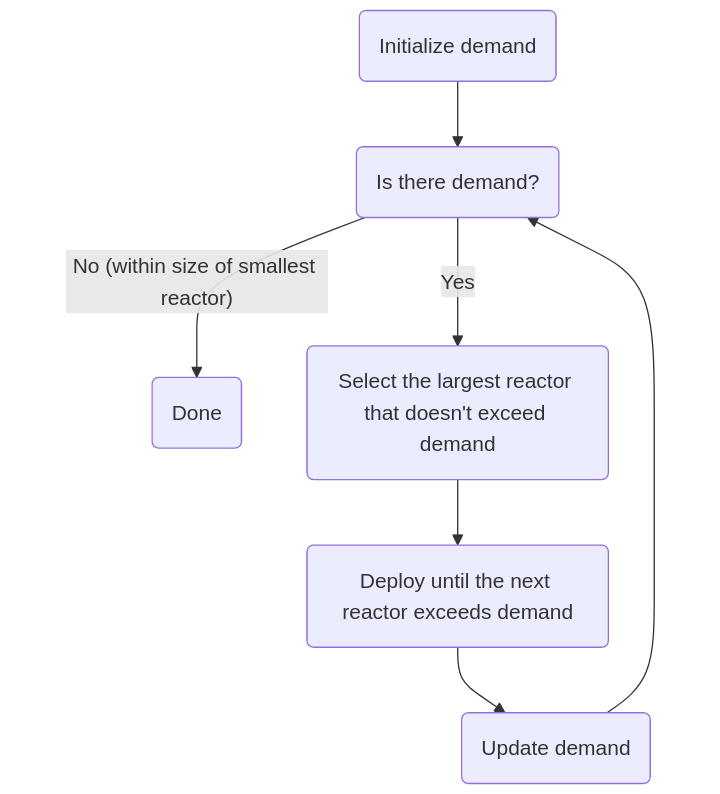
\includegraphics[scale=0.3]{images/schemes/greedy_diagram.png}
    \caption{Greedy deployment diagram.}
    \label{fig:greedy_diagram}
\end{figure}

The \textit{greedy deployment} does not attempt to capture the complexity of the deployment problem but rather to explore the implications of deploying a certain number of reactors. The scheme could mirror large actors in a market, but is likely not realistic. The scheme will deploy reactors until the demand is met within the amount of the smallest capacity reactor. Sections \ref{sec:greedy_reactors}, \ref{sec:greedy_swu}, \ref{sec:greedy_fresh}, and \ref{sec:greedy_used} show the \textit{greedy deployment} results for the \textit{no growth} scenario and the \textit{double nuclear by 2050} scenario.

\subsection{Number of Reactors}
\label{sec:greedy_reactors}

As Section \ref{fig:dep_goals} mentions, one difference between the \textit{no growth} scenario and the doubling scenario is that the transition for the \textit{no growth} scenario will begin closer to 2050 instead of 2030. This trend is reflected in Figures \ref{fig:greedy_mf_reactors} and \ref{fig:greedy_of_reactors}, where the \glspl{mmr}, \glspl{xe}, and AP1000s start as the existing \gls{lwr} fleet is retired. Comparing fuel regimes, Figures \ref{fig:greedy_mf_ng_reactors} and \ref{fig:greedy_of_ng_reactors} are identical, which typifies the impact of the delayed transition in the \textit{no growth} scenario.

% Show total number of reactors multi-fuel

\begin{figure}[H]
    \subfloat[No Growth. \label{fig:greedy_mf_ng_reactors}]{%
      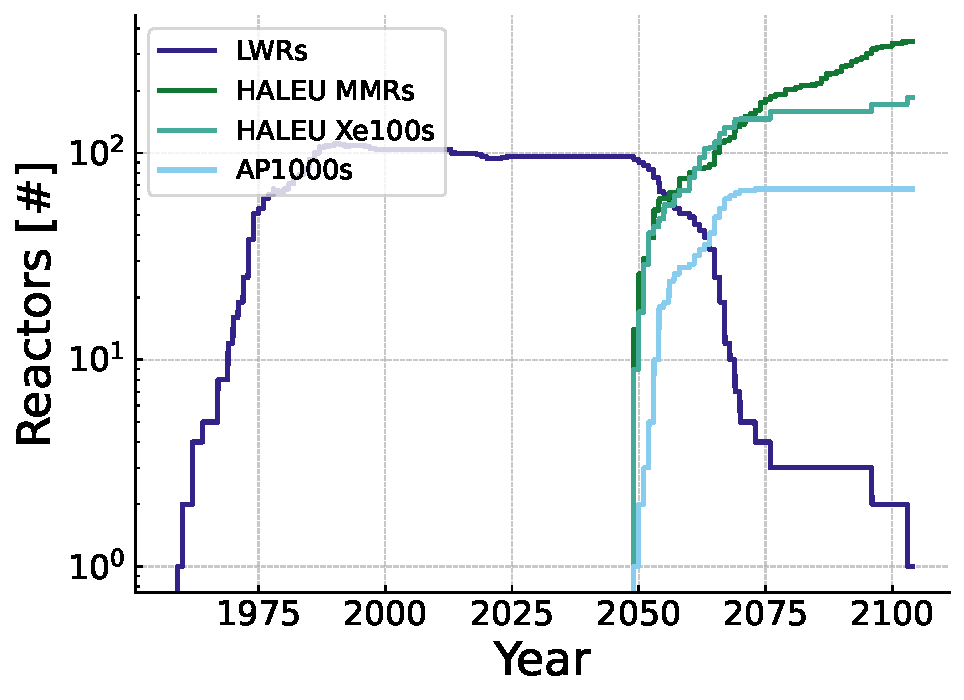
\includegraphics[width=0.495\textwidth]{images/results/reactors/multi_dgng_reactors.pdf}
   }
    \hfill
    \subfloat[Double. \label{fig:greedy_mf_d2_reactors}]{%
      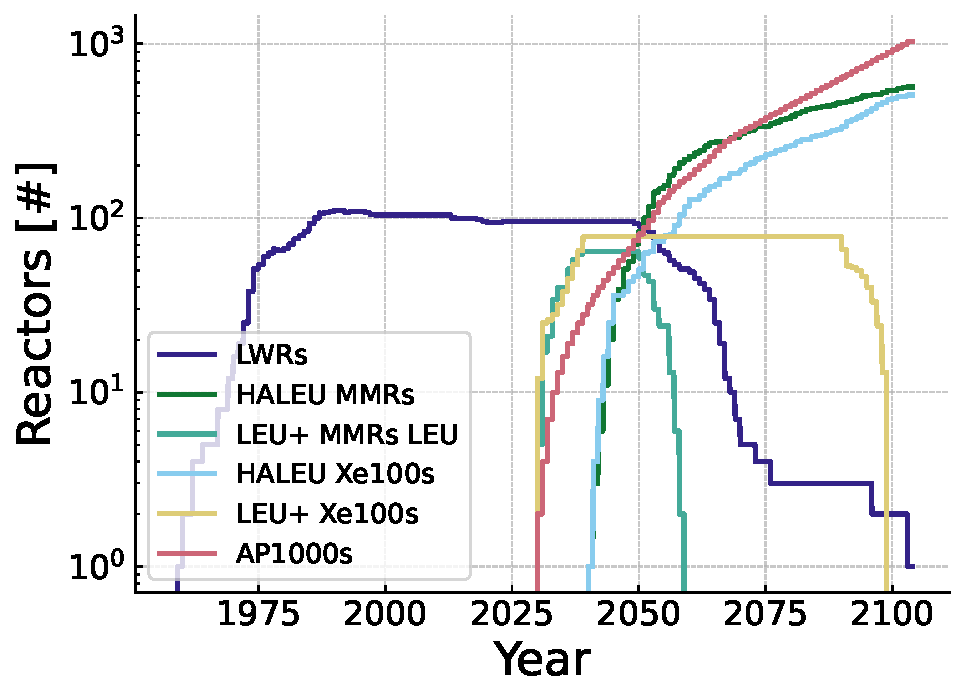
\includegraphics[width=0.495\textwidth]{images/results/reactors/multi_dg2_reactors.pdf}
   }
    \caption{Greedy multi-fuel reactor deployment.}
    \label{fig:greedy_mf_reactors}
\end{figure}

% talk about the rate of deployment
A direct consequence of the \textit{greedy deployment} scheme is that, in the doubling scenario, the AP1000 is deployed the most over time, whereas the \textit{no growth} scenario shows the opposite. Another consequence of the deployment scheme is that the deployment rate for the single-fuel regime compared with the multi-fuel regime is identical, and future work could investigate further implications of transitioning from one fuel type to another regarding operation. Simply meeting energy demand is not how utilities make decisions and is not the intended use case of the broad generation of new nuclear reactors, so this is an upper-bounding case for the energy demand met by designs like the \gls{mmr} or \gls{xe}.


\begin{figure}[H]
  \subfloat[No Growth. \label{fig:greedy_of_ng_reactors}]{%
    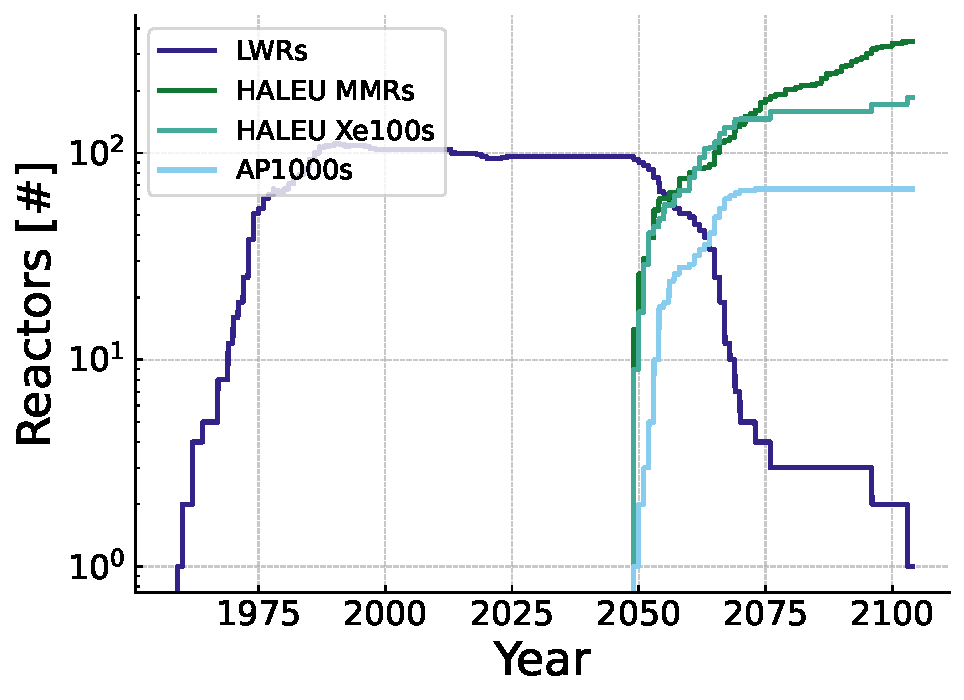
\includegraphics[width=0.495\textwidth]{images/results/reactors/one_dgng_reactors.pdf}
 }
  \hfill
  \subfloat[Double. \label{fig:greedy_of_d2_reactors}]{%
    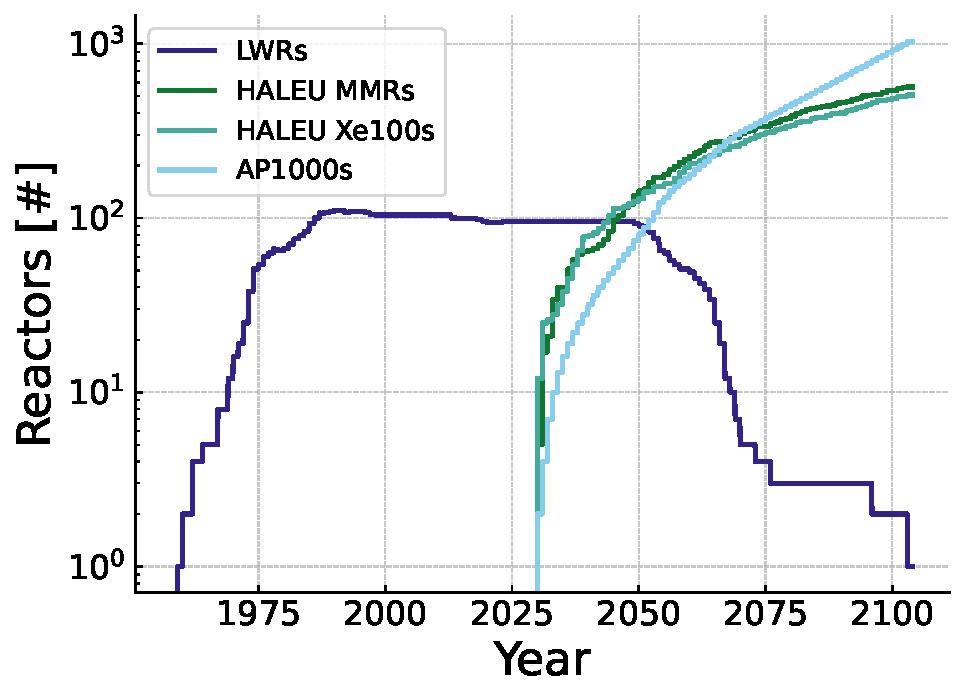
\includegraphics[width=0.495\textwidth]{images/results/reactors/one_dg2_reactors.pdf}
 }
  \caption{Greedy single-fuel reactor deployment.}
  \label{fig:greedy_of_reactors}
\end{figure}

Table \ref{tab:greedy_reac_avg} shows how the average number of reactors by design is not influenced by the interstitial period included in this thesis. Compared to the \textit{no growth} scenario, the \textit{double by 2050} scenario shows a significant increase in the average number of each design operating across the 2030-2104 timeline. Consequently, the average number of the AP1000s increases by 757\% between the two growth scenarios, which is the largest increase of any design. The \gls{xe} reactors show the second largest increase at 163\%, followed by the \gls{mmr} at 109\%.

\begin{table}[H]
  \centering
  \caption{Average greedy total operating reactors by design.}
  \label{tab:greedy_reac_avg}
  \begin{tabular}{l c c c c}
     \hline
     Scenario & No Growth, Single & No Growth, Multiple & Double, Single & Double, Multiple  \\
     \hline
     \gls{haleu} fueled MMRs      & 131.613 & 131.613 & 274.493 & 257.427 \\
     \gls{leup} fueled MMRs       & --      & --      & --      & \textcolor{white}{0}17.067 \\
     \gls{haleu} fueled \gls{xe}s & \textcolor{white}{0}94.04   & \textcolor{white}{0}94.04   & 246.88  & 184.48 \\
     \gls{leup} fueled \gls{xe}s  & --      & --      & --      & \textcolor{white}{0}62.4 \\
     \gls{leu} fueled AP1000      & \textcolor{white}{0}38.667  & \textcolor{white}{0}38.667  & 331.387 & 331.387 \\
     \hline
  \end{tabular}
\end{table}




\subsection{SWU Results}
\label{sec:greedy_swu}

% talk about the types of category facility
In Figure \ref{fig:swu_yearly_greedy}, the yearly \gls{swu} demand periodically spikes as the demand for enrichment services grows to meet the fuel demand for the fleet. When reactors begin operation in the depicted \textit{no growth} scenario around 2050, the \gls{swu} demand for the AP1000 peaks above the other two reactors, while the demand from \glspl{xe} exceeds the demand from \glspl{mmr}. This trend is exacerbated in the \textit{double by 2050} scenarios shown in Figures \ref{fig:greedy_mf_d2_swu} and \ref{fig:greedy_of_d2_swu}, where the \gls{swu} for AP1000 \gls{leu} fuel rises quickly and eventually exceeds the total \gls{swu} for the existing fleet.

% talk about the SWU capacity

% show the total SWU capacity

\begin{figure}[H]
    \centering
    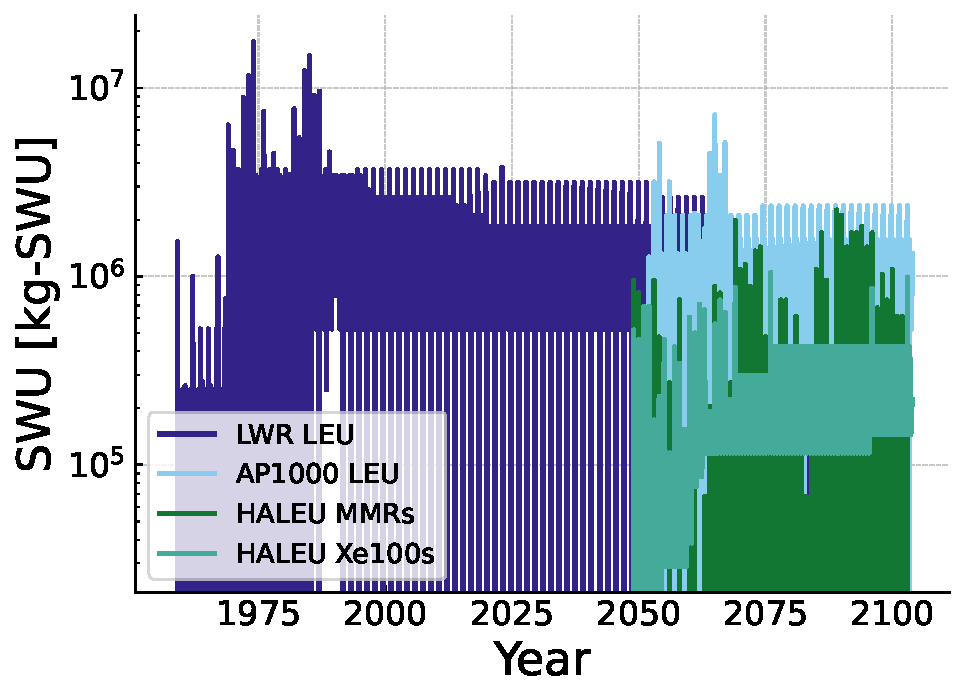
\includegraphics[scale=0.7]{images/results/swu/multi_dgng_swu_by_fuel.pdf}
    \caption{Greedy yearly SWU capacity multi-fuel, no growth scenario.}
    \label{fig:swu_yearly_greedy}
\end{figure}

As the features of the yearly data are regular and dictated by the reactor's cycle, Figures \ref{fig:greedy_mf_swu} and \ref{fig:greedy_of_swu} visualize the total cumulative \gls{swu} demand.

\begin{figure}[H]
  \subfloat[No Growth. \label{fig:greedy_mf_ng_swu}]{%
    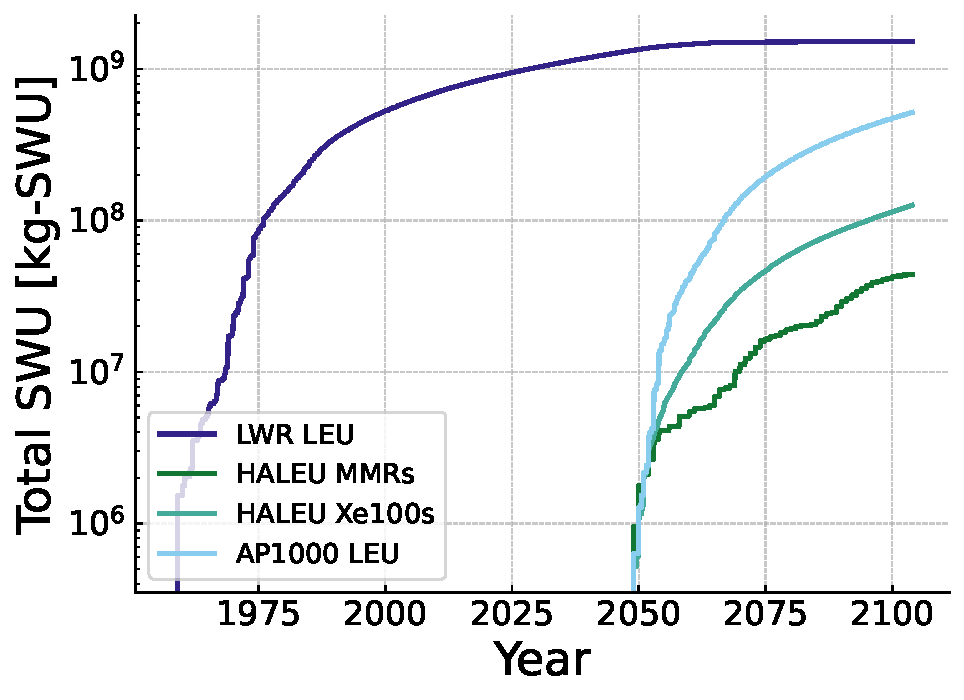
\includegraphics[width=0.495\textwidth]{images/results/swu/multi_dgng_swu_cumulative_by_fuel.pdf}
 }
  \hfill
  \subfloat[Double. \label{fig:greedy_mf_d2_swu}]{%
    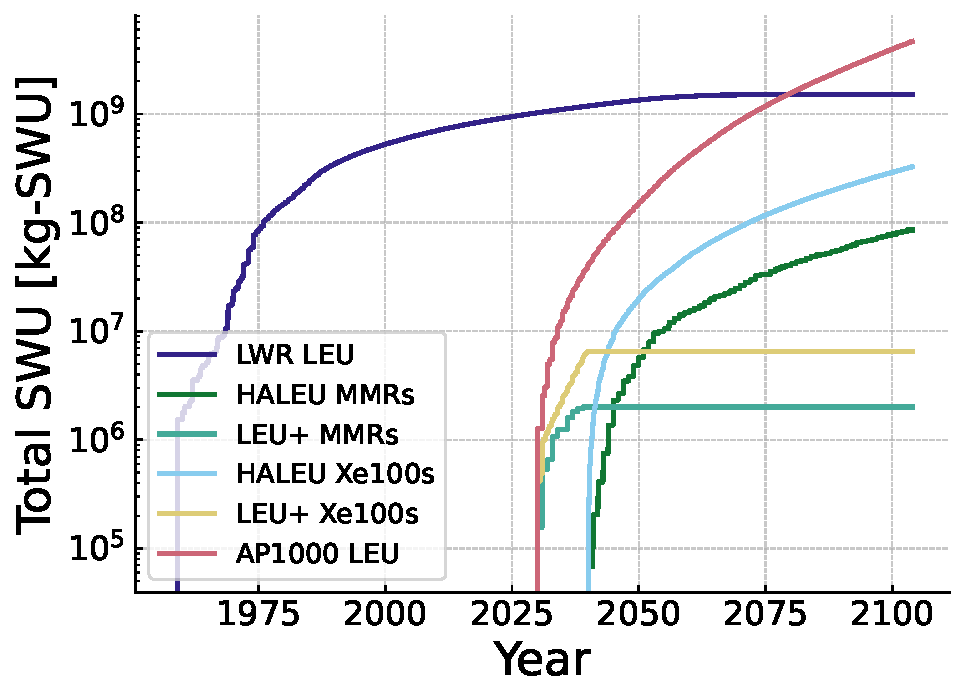
\includegraphics[width=0.495\textwidth]{images/results/swu/multi_dg2_swu_cumulative_by_fuel.pdf}
 }
  \caption{Greedy multi-fuel SWU.}
  \label{fig:greedy_mf_swu}
\end{figure}


% talk about international trade

\begin{figure}[H]
  \subfloat[No Growth. \label{fig:greedy_of_ng_swu}]{%
    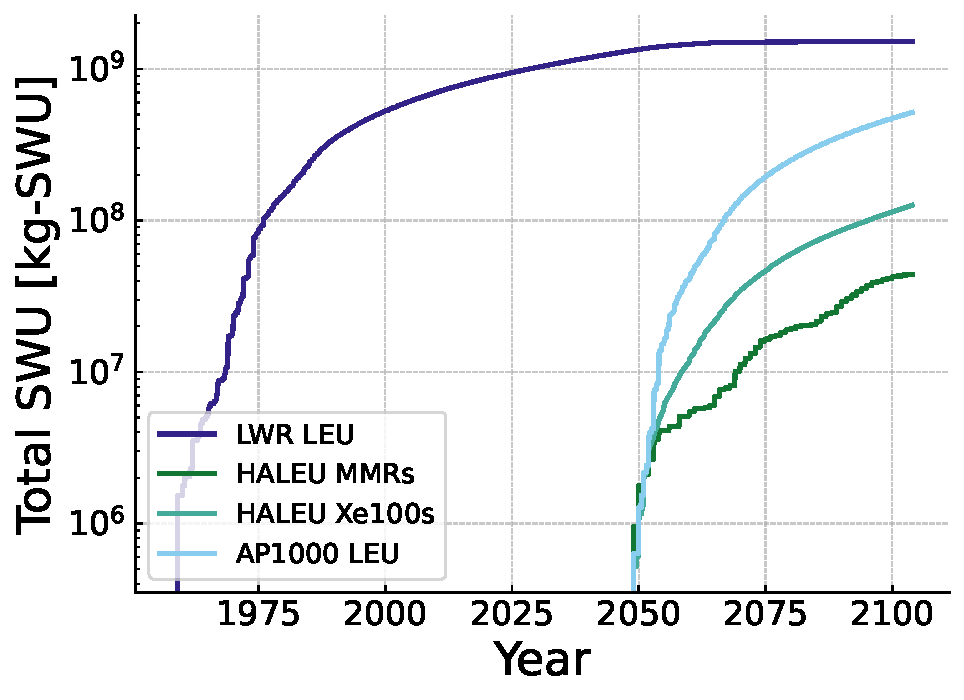
\includegraphics[width=0.495\textwidth]{images/results/swu/one_dgng_swu_cumulative_by_fuel.pdf}
 }
  \hfill
  \subfloat[Double. \label{fig:greedy_of_d2_swu}]{%
    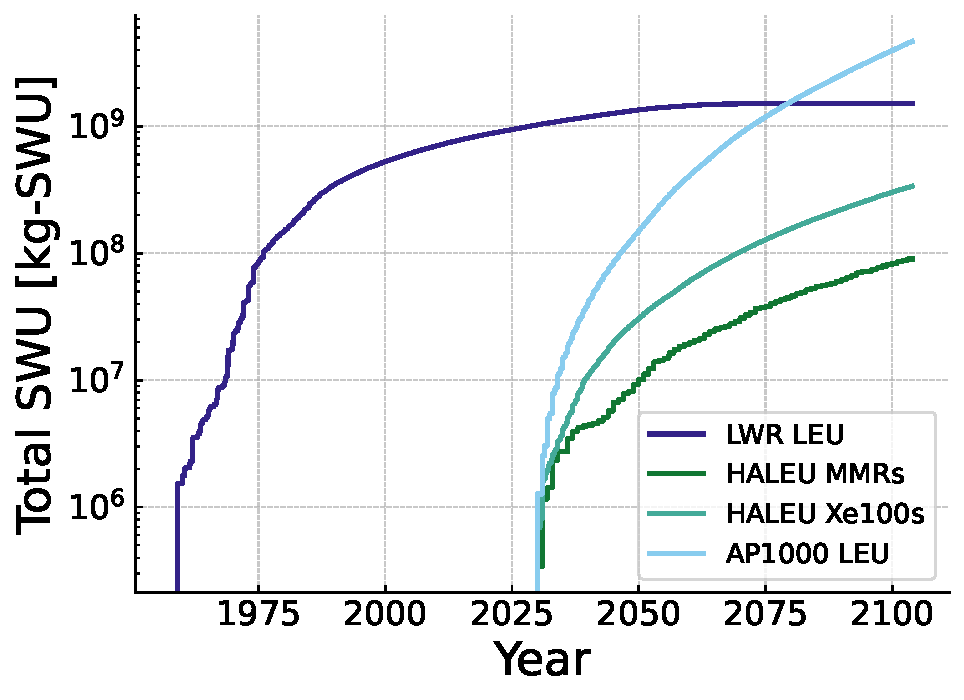
\includegraphics[width=0.495\textwidth]{images/results/swu/one_dg2_swu_cumulative_by_fuel.pdf}
 }
  \caption{Greedy single-fuel SWU.}
  \label{fig:greedy_of_swu}
\end{figure}

Table \ref{tab:greedy_swu_avg} shows how the \gls{swu} demand for the \gls{mmr} and \gls{xe} reactors are the same in the single and multi-fuel regimes for the \textit{no growth} scenarios, consistent with the reactor deployment trends in Section \ref{sec:greedy_reactors}. The \gls{swu} demand for the AP1000s increases by 800\% from the \textit{no growth} scenario to the \textit{double by 2050} scenario, again consistent with the reactor deployment trends in the previous section. The \gls{swu} demand for \gls{xe} \gls{haleu} increases by 167\%, while the \gls{swu} demand for \gls{mmr} \gls{haleu} increases by 105\% from the \textit{no growth} scenario to the \textit{double by 2050} scenario.

\begin{table}[H]
  \centering
  \caption{Average greedy yearly SWU by design in k\gls{swu}.}
  \label{tab:greedy_swu_avg}
  \begin{tabular}{l c c c c}
     \hline
     Scenario & No Growth, Single & No Growth, Multiple & Double, Single & Double, Multiple  \\
     \hline
     \gls{mmr} \gls{haleu}   & \textcolor{white}{00}48.699  & \textcolor{white}{00}48.699  & \textcolor{white}{00}99.974   & \textcolor{white}{00}95.127   \\
     \gls{mmr} \gls{leup}    & --      & --      & --       & \textcolor{white}{000}2.228    \\
     \gls{xe} \gls{haleu}    & \textcolor{white}{0}139.926 & \textcolor{white}{0}139.926 & \textcolor{white}{0}374.323  & \textcolor{white}{0}362.312  \\
     \gls{xe} \gls{leup}     & --      & --      & --       & \textcolor{white}{000}7.227    \\
     AP1000 \gls{leu}        & \textcolor{white}{0}573.989 & \textcolor{white}{0}573.989 & 5167.815 & 5167.815 \\
     \hline
  \end{tabular}
\end{table}



\subsection{Fresh Fuel Results}
\label{sec:greedy_fresh}

% talk about the types of fuel
Figures \ref{fig:greedy_mf_fresh} and \ref{fig:greedy_of_fresh} show the fresh fuel demand for the reactors in the \textit{no growth} and \textit{double by 2050} scenarios. The fresh fuel curves in each scenario follow the same pattern as the reactor deployment curves, as \cyclus supplies fuel to each of the reactors as it is deployed.

% show total fresh fuel

\begin{figure}[H]
  \subfloat[No Growth. \label{fig:greedy_mf_ng_fresh}]{%
    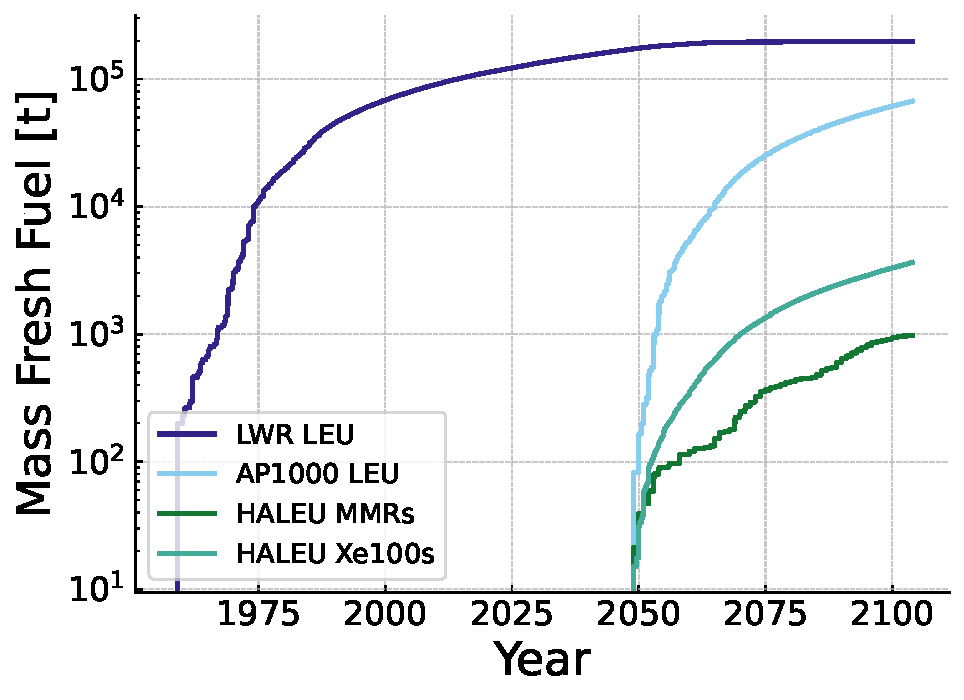
\includegraphics[width=0.495\textwidth]{images/results/fresh/multi_dgng_fresh_fuel_cumulative_by_fuel.pdf}
 }
  \hfill
  \subfloat[Double. \label{fig:greedy_mf_d2_fresh}]{%
    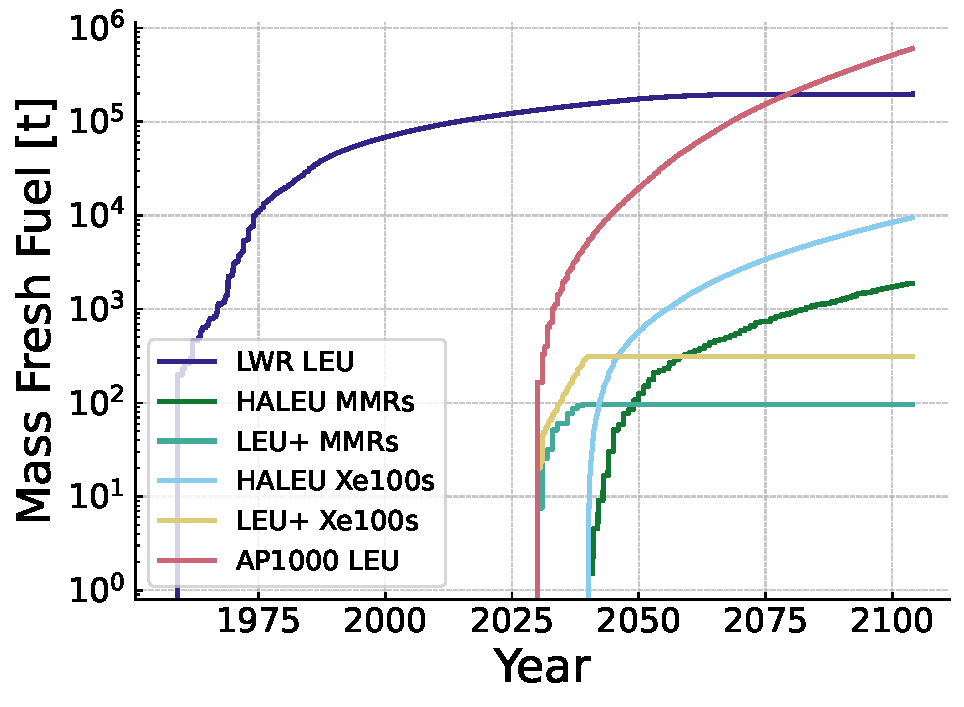
\includegraphics[width=0.495\textwidth]{images/results/fresh/multi_dg2_fresh_fuel_cumulative_by_fuel.pdf}
 }
  \caption{Greedy multi fresh fuel demanded.}
  \label{fig:greedy_mf_fresh}
\end{figure}

% talk about transportation of fuel


\begin{figure}[H]
  \subfloat[No Growth. \label{fig:greedy_of_ng_fresh}]{%
    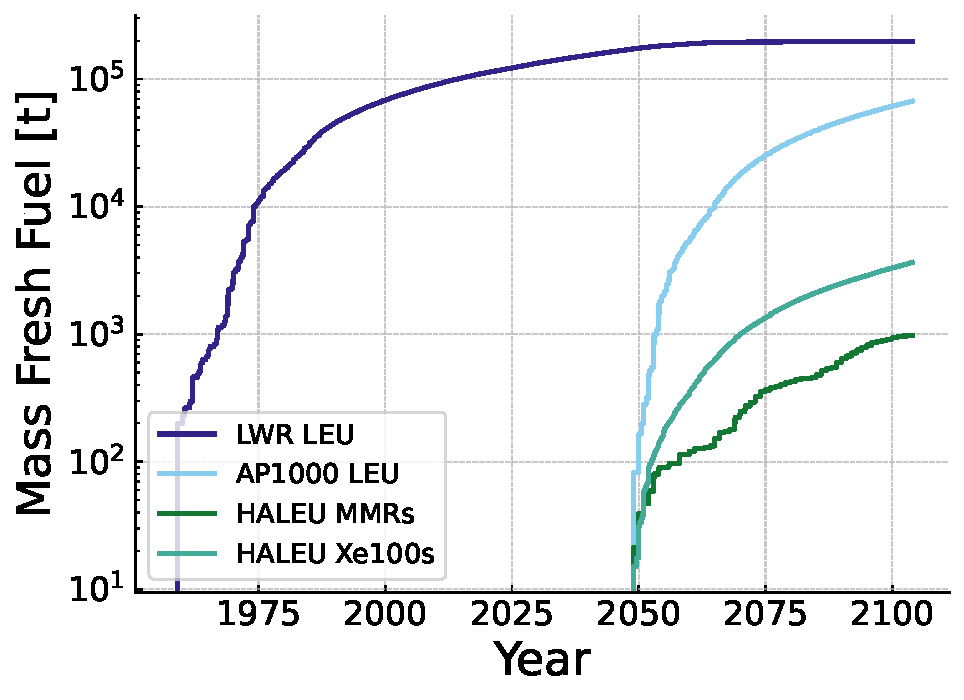
\includegraphics[width=0.495\textwidth]{images/results/fresh/one_dgng_fresh_fuel_cumulative_by_fuel.pdf}
 }
  \hfill
  \subfloat[Double. \label{fig:greedy_of_d2_fresh}]{%
    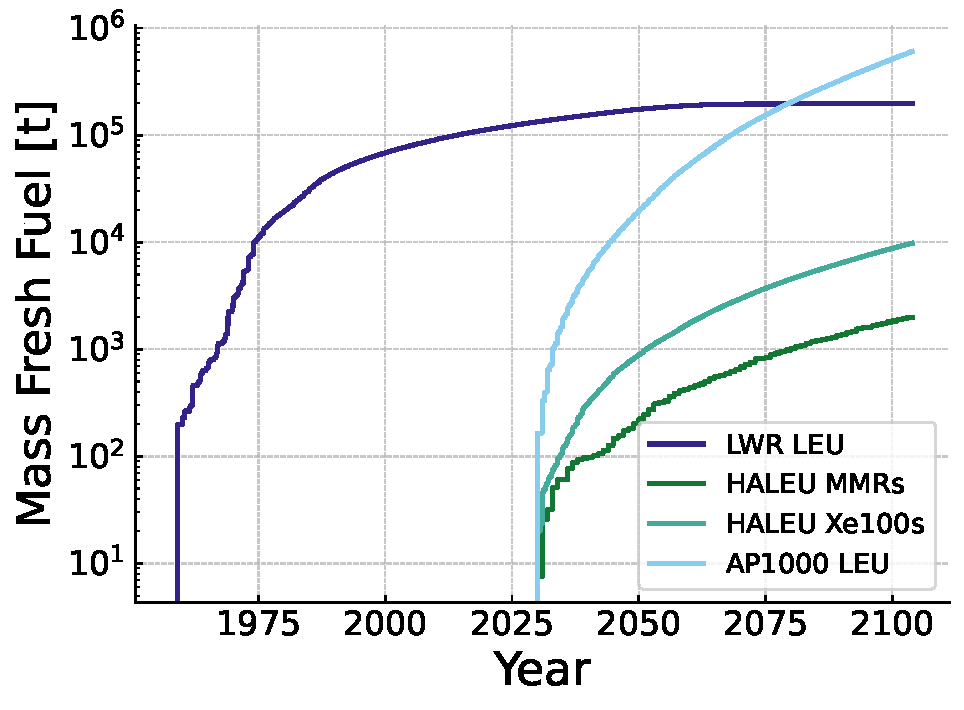
\includegraphics[width=0.495\textwidth]{images/results/fresh/one_dg2_fresh_fuel_cumulative_by_fuel.pdf}
 }
  \caption{Greedy single fresh fuel demanded.}
  \label{fig:greedy_of_fresh}
\end{figure}

Table \ref{tab:greedy_fresh_avg} quantifies the average yearly fresh fuel demand by design in the \textit{no growth} and \textit{double by 2050} scenarios. The AP1000 \gls{leu} shows the largest increase in fresh fuel demand from the \textit{no growth} scenario to the \textit{double by 2050} scenario at 800\%, followed by the \gls{xe} \gls{haleu} at 159\%. The \gls{mmr} \gls{haleu} reactors show the smallest increase in fresh fuel demand at 105\%.


\begin{table}[H]
  \centering
  \caption{Average greedy yearly fresh fuel by design in tonnes.}
  \label{tab:greedy_fresh_avg}
  \begin{tabular}{l c c c c}
     \hline
     Scenario & No Growth, Single & No Growth, Multiple & Double, Single & Double, Multiple  \\
     \hline
     \gls{mmr} \gls{haleu}   & \textcolor{white}{00}1.079    & \textcolor{white}{00}1.079   & \textcolor{white}{00}2.216    & \textcolor{white}{00}2.108    \\
     \gls{mmr} \gls{leup}    & --       & --      & --       & \textcolor{white}{00}0.107    \\
     \gls{xe} \gls{haleu}    & \textcolor{white}{00}4.059    & \textcolor{white}{00}4.059   & \textcolor{white}{0}10.859   & \textcolor{white}{0}10.511   \\
     \gls{xe} \gls{leup}     & --       & --      & --       & \textcolor{white}{00}0.348    \\
     AP1000 \gls{leu}        & \textcolor{white}{0}74.636   & \textcolor{white}{0}74.636  & 671.976  & 671.976  \\
     \hline
  \end{tabular}
\end{table}



\subsection{Used Fuel Results}
\label{sec:greedy_used}

Figures \ref{fig:greedy_mf_used} and \ref{fig:greedy_of_used} describe the used fuel demand for the reactors in the \textit{no growth} and \textit{double by 2050} scenarios. The used fuel curves in each scenario lag the reactor deployment curves, as \cyclus removes the used fuel after the appropriate number of cycles from each operating and eventually decommissioning reactor.

% show total used fuel
\begin{figure}[H]
  \subfloat[No Growth. \label{fig:greedy_mf_ng_used}]{%
    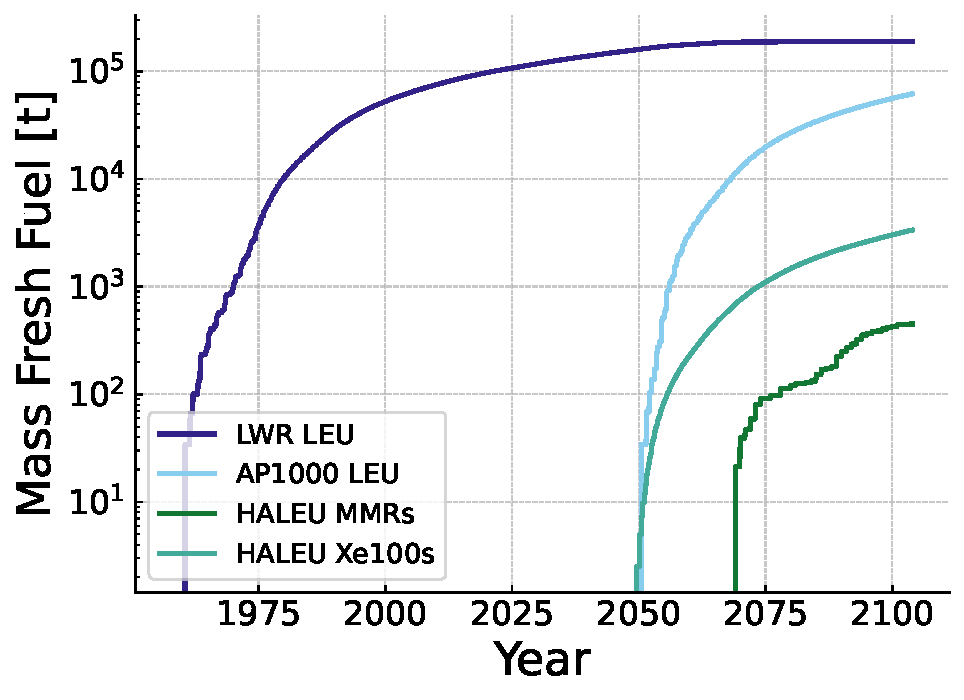
\includegraphics[width=0.495\textwidth]{images/results/used/multi_dgng_used_fuel_cumulative_by_fuel.pdf}
 }
  \hfill
  \subfloat[Double. \label{fig:greedy_mf_d2_used}]{%
    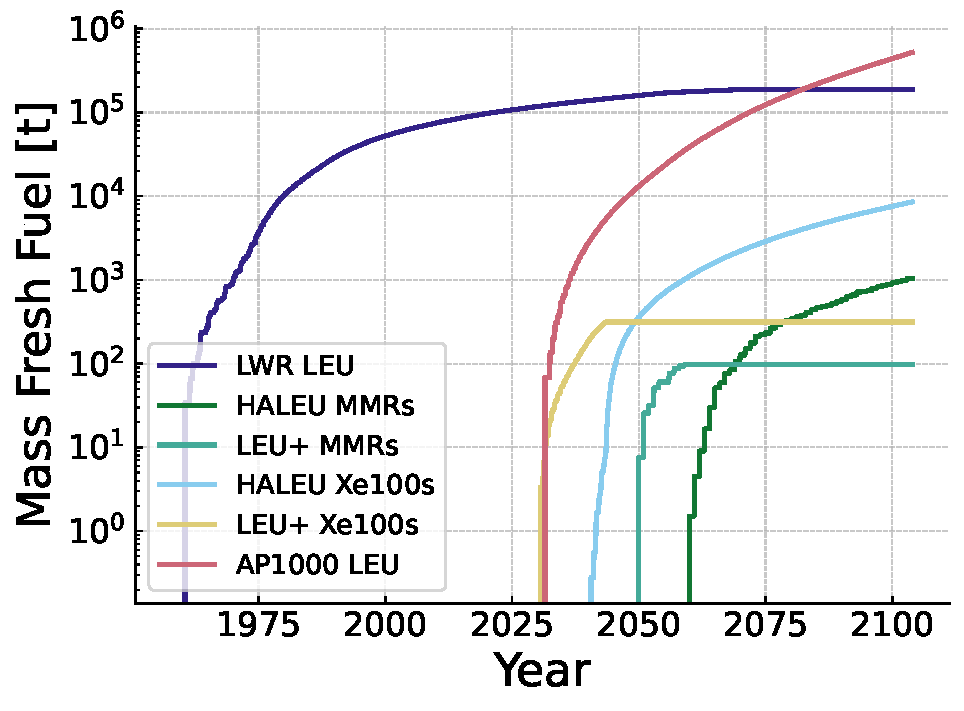
\includegraphics[width=0.495\textwidth]{images/results/used/multi_dg2_used_fuel_cumulative_by_fuel.pdf}
 }
  \caption{Greedy multi used fuel accumulation.}
  \label{fig:greedy_mf_used}
\end{figure}


\begin{figure}[H]
  \subfloat[No Growth. \label{fig:greedy_of_ng_used}]{%
    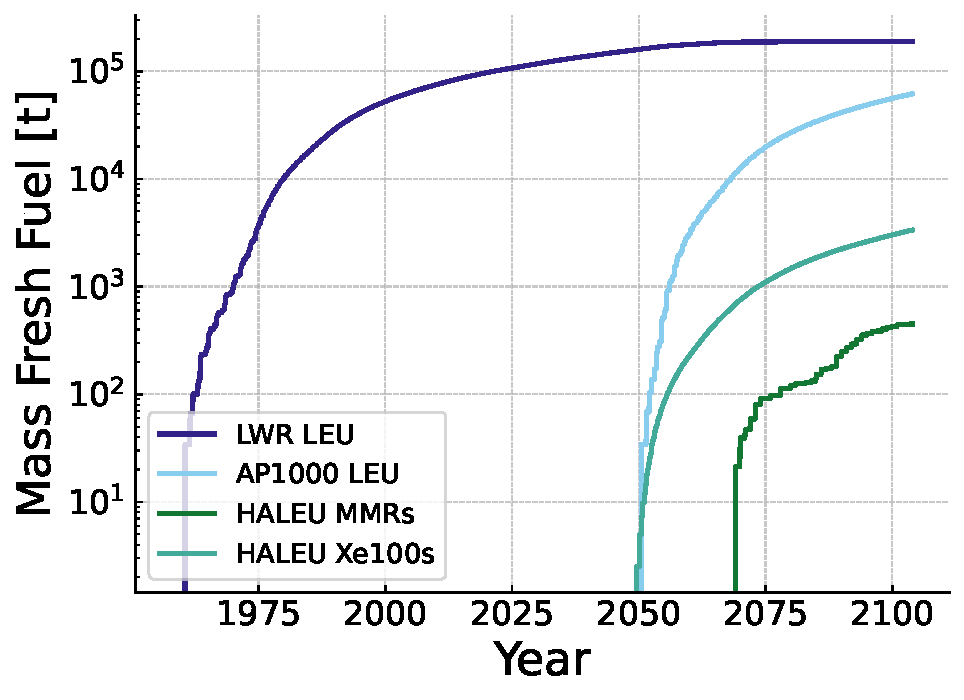
\includegraphics[width=0.495\textwidth]{images/results/used/one_dgng_used_fuel_cumulative_by_fuel.pdf}
 }
  \hfill
  \subfloat[Double. \label{fig:greedy_of_d2_used}]{%
    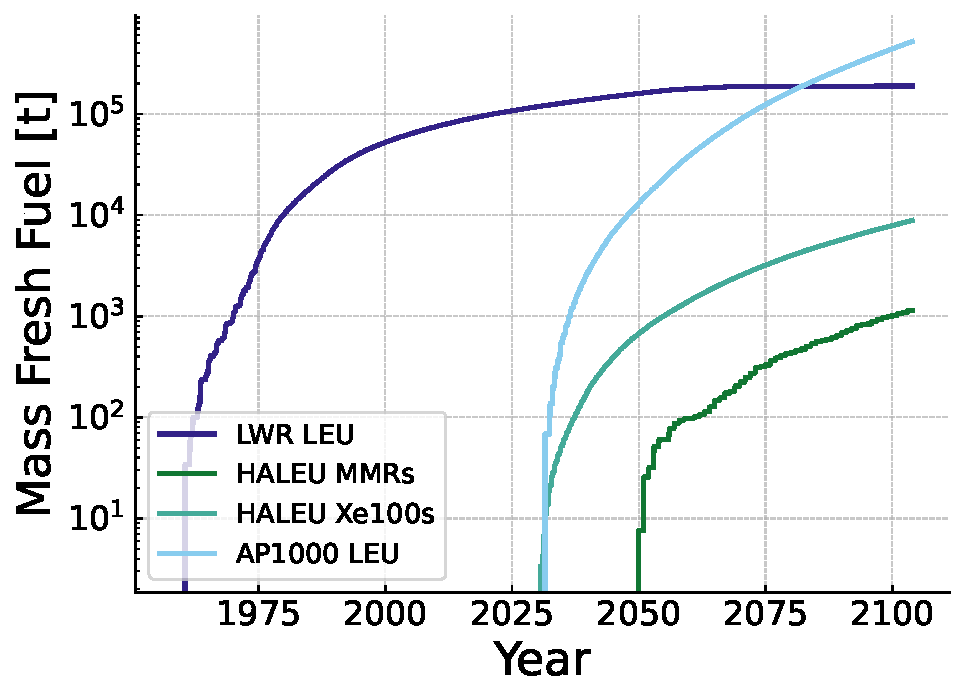
\includegraphics[width=0.495\textwidth]{images/results/used/one_dg2_used_fuel_cumulative_by_fuel.pdf}
 }
  \caption{Greedy single used fuel accumulation.}
  \label{fig:greedy_of_used}
\end{figure}

Table \ref{tab:greedy_used_avg} itemizes the average yearly used fuel by design in the \textit{no growth} and \textit{double by 2050} scenarios. The AP1000 \gls{leu} shows the largest increase in used fuel demand from the \textit{no growth} scenario to the \textit{double by 2050} scenario at 743\%, followed by the \gls{xe} \gls{haleu} at 164\%. The \gls{mmr} \gls{haleu} reactors show the smallest increase in used fuel demand at 154\%.


\begin{table}[H]
  \centering
  \caption{Average greedy yearly used fuel by design in tonnes.}
  \label{tab:greedy_used_avg}
  \begin{tabular}{l c c c c}
     \hline
     Scenario & No Growth, Single & No Growth, Multiple & Double, Single & Double, Multiple  \\
     \hline
     \gls{mmr} \gls{haleu}   & \textcolor{white}{00}0.499    & \textcolor{white}{00}0.499   & \textcolor{white}{00}1.267    & \textcolor{white}{00}1.160    \\
     \gls{mmr} \gls{leup}    & --       & --      & --       & \textcolor{white}{00}0.107    \\
     \gls{xe} \gls{haleu}    & \textcolor{white}{00}3.714    & \textcolor{white}{00}3.715   & \textcolor{white}{00}9.826    & \textcolor{white}{00}9.477    \\
     \gls{xe} \gls{leup}     & --       & --      & --       & \textcolor{white}{00}0.348    \\
     AP1000 \gls{leu}        & \textcolor{white}{0}68.496   & \textcolor{white}{0}68.496  & 577.484  & 577.484  \\
     \hline
  \end{tabular}
\end{table}


% talk about repositories